\chapter{TCP/IP stack}

\section{TCP/IP stack characteristics}

As a simplified OSI model, the TCP/IP stack allows for simple classification of the protocols based on their functions and abstraction level. Lower layers focus primarily on the hardware aspects, while higher levels target functionalities. This chapter discusses each layer of the TCP/IP stack in a descending order.

\section{Application layer}

This layer serves as an interface between computer software and the remaining TCP/IP stack layers. Depending on the functionality provided by the end program, application layer puts forward protocols of various uses \cite{tcpip:layers}:

\begin{itemize}
	\item [1)] HTTP, HTTPS (\emph{Hypertext Transfer Protocol}, \emph{Hypertext Transfer Protocol Secure}) -- protocols responsible for transmission of WWW forms between the server and the end user, in non-encrypted and encrypted version respectively \cite{http};
	\item [2)] FTP, TFTP, NFS (\emph{File Transfer Protocol}, \emph{Trivial File Transfer Protocol}, \emph{Network File System}) -- protocols for transmitting files between two devices via the Internet;
	\item [3)] SMTP, POP3, IMAP (\emph{Simple Mail Transfer Protocol}, \emph{Post Office Protocol 3}, \emph{Internet Message Access Protocol}) -- a group of protocols responsible for e-mail communication \cite{ibm:smtp}\cite{uci:pop3};
	\item [4)] Telnet -- a protocol for remote access into different computer, allowing for logging in and transmitting input from host to the remote client \cite{slownik:telnet};
	\item [5)] SNMP (\emph{Simple Network Management Protocol}) -- protocol for managing devices connected to the network, which are equipped with SNMP agent. It allows for the remote configuration of network devices such as routers, servers and switches \cite{ibm:snmp};
	\item [6)] DNS (\emph{Domain Name System}) - a protocol responsible for translating the domain names into IP addresses of the servers hosting given website or service;
	\item [7)] IRC (\emph{Internet Relay Chat}) -- a client-server model protocol which allows live communication via text communicators (\emph{chats}) \cite{irc};
	\item [8)] DGCP (\emph{Dynamic Host Configuration Protocol}) -- it is responsible for dynamically configuring the end devices connected to a computer network through assigning them so called dynamic IP address based on the available address pool.
\end{itemize}

Regardless of the different form of information created by the aforementioned protocols, 

Pomimo różnej konstrukcji informacji wytworzonej przez wymienione protokoły, w niższych warstwach są one uniwersalnie interpretowane jako sekcja danych, która następnie jest obudowywana przez protokoły warstw niższych w procesie tzw. enkapsulacji. Do komunikacji pomiędzy warstwą aplikacji a warstwą transportową wykorzystywane są tzw. gniazda sieciowe (ang. \emph{Internet Sockets}) będące konstrukcjami programowymi zawierającymi informacje o adresie IP, numerze portu i wykorzystywanym protokole \cite{tcpip:layers}.

\section{Transport layer}

Here data received from the application layer is divided into a series of packets and wrapped in a header containing information such as the number or the port of the sender and receiver, which is important in order to determine, which protocol of the application layer should get the message on the receiver end. Protocols used in this layer determine the characteristics of the transmission. The main protocol of this layer are TCP and UDP.

\begin{figure}[!ht]
    \centering
    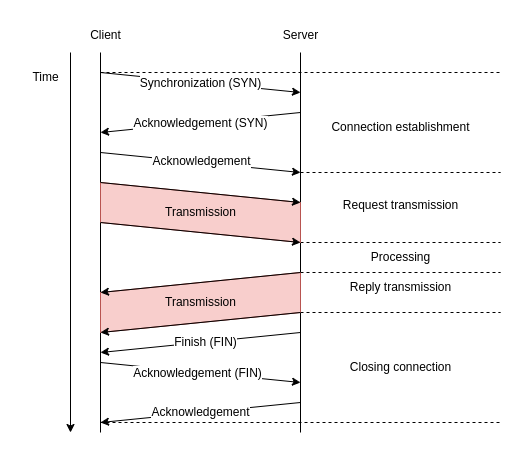
\includegraphics[width=90mm]{Rysunki/Rozdzial3/tcptransmission.png}
    \caption{TCP transmission diagram}
    \label{fig:my_label}
\end{figure}

TCP (\emph{Transmission Control Protocol}) is a connection oriented protocol, which means that at the start of the transmission, a session between the transmitter and the receiver is created. Additionally, it is characterized by reliability, due to the requirement of getting an acknowledgement for each transmitted packet, and performing a retransmission in case of transmission errors or lack of acknowledgement. This characteristics is especially important in case of exchanging data, which integrity plays a key role, such as files or e-mail messages. Primary protocols in the application layer which utilize TCP transmission are: HTTP, HTTPS, FTP, SMTP and Telnet \cite{tcpip:layers}. The flow of a singular transmission is presented on figure 3.1.

UDP (\emph{User Datagram Protocol}), on contrary to the TCP, is not a connection oriented protocol and it does not perform any retransmissions. This means that transmitting a message using the UDP protocol does not guarantee that it reach the recipient. Additionally, the order in which the packets are received does not need to reflect the order of their transmission, which requires sorting by the recipient devices. The advantage of UDP protocol however is increased speed of the transmission thanks to significant simplification of utilized mechanisms. This comes especially handy in case of services, where losing singular packets is not a problem, and keeping a low latency is of much bigger importance. This especially concerns voice transmission, and online video games. Example protocols utilizing UDP transmission are: DNS, DHCP, TFTP, SNMP, RIP and VOIP \cite{tcpip:layers}. The flow of singular transmission was presented on figure 3.2. 


\begin{figure}[!ht]
    \centering
    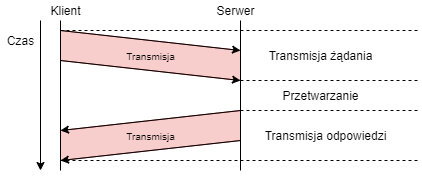
\includegraphics[width=100mm]{Rysunki/Rozdzial3/udptransmission.png}
    \caption{UDP transmission diagram}
    \label{fig:my_label}
\end{figure}

\section{Network layer}

In this layer, the transmission frame is wrapped in address fields containing the IP addresses of the sender and the recipient. Their presence is important due to the method of routing data in the Internet, which bases on passing the packet between subsequent devices until it reaches the recipient. Network devices know know on which port the packet should be forwarded thanks to their configuration. The IP protocol used for addressing is available in version IPv4 and IPv6, which differ in the length of the addresses, the manner of addressing networks and subnetworks, and translation of the addresses between public and private in case of IPv4, or lack thereof in case of IPv6.

Other than the IP protocol, the network layer offers following protocols:

\begin{itemize}
	\item [1)] ARP (\emph{Address Resolution Protocol}) -- it serves the purpose of acquiring the MAC address of the device with corresponding IP address;
	\item [2)] RARP (\emph{Reverse Address Resolution Protocol}) -- allows for acquiring the IP address of a device based on its MAC address;
	\item [3)] ICMP (\emph{Internet Control Message Protocol}) -- a protocol allowing to oversee the state of given computer network.
\end{itemize}

The necessity of use of protocols which give access to MAC addresses based on IP addresses arises from the difference in addressing between the network layer, which uses IP addresses, and network access layer, which uses MAC addresses. During the transmission of a packet, each of the intermediary devices performs packet decapsulation to the form available in network layer, and subsequently makes the decision whether the packet should be forwarded further based on the IP address. In case of the need to forward the message to another device, it is encapsulated again with information about MAC addresses in the network access layer. In the opposite case the packet is forwarded to the higher layers. Figure 3.3. shows the layer diagram, in which a packet is processed during transmission between two intermediary devices.  

\begin{figure}[!ht]
    \centering
    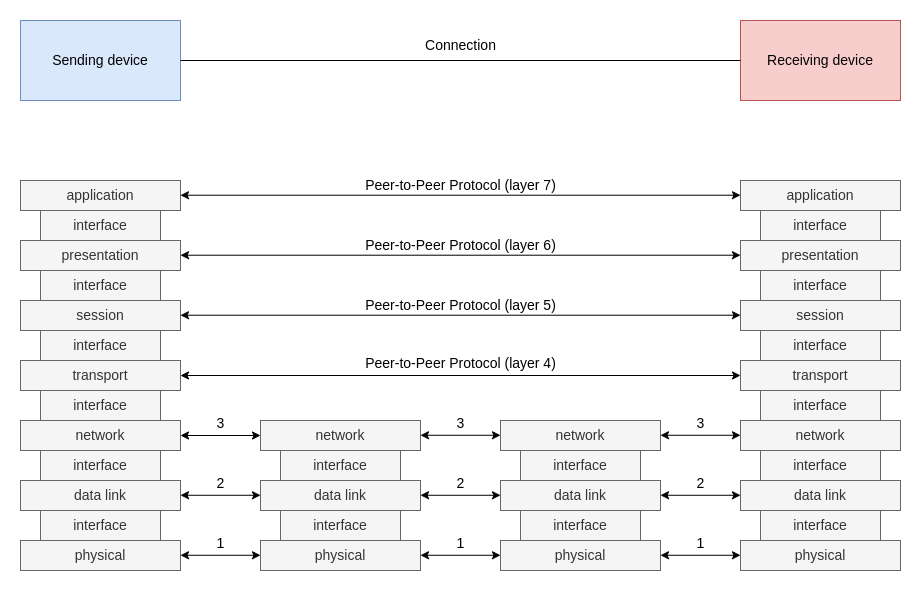
\includegraphics[width=155mm]{Rysunki/Rozdzial3/osi_route.png}
    \caption{Packet path diagram in the OSI model - Computer Notes}
    \label{fig:my_label}
\end{figure}

\section{Network access layer}

The layer responsible for preparing the packets for transmission using the physical medium, and carrying out the transmission. Both in case of wired and wireless networks, following sublayers can be identified:

\begin{itemize}
	\item [1)] LLC (\emph{Logic Link Control}) -- concatenates the frame with information about the protocol used in transport layer, in order to allow the recipient device to correctly interpret the received packet;
	\item [2)] MAC (\emph{Media Access Control}) -- creates the physical addresses sections in the Ethernet frame, storing MAC address of the sender and either the recipient, or intermediary router. In case of intermediary routers, the recipient address is updated by the router during the forwarding of the packet;
	\item [3)] PHY (\emph{Physical}) -- consists of elements of the physical medium for transmission, such as transmission wires, antennas and transceivers;
\end{itemize}

Two primary connectivity methods can be distinguished on the physical interface level: wired and wireless/

\subsection{Wired connectivity}

In order to connect devices in a wired manner, an UTP cable is commonly used, which utilizes the 8P8C connector, commonly incorrectly called RJ-45 due to very similar shape (RJ-45 connector has additional extrusion) \cite{8p8c}. The 8P8C is an 8-pin connector, which has 4 pairs of wires marked by straight and dashed isolation colors. It allows for connecting two devices via Point-to-Point method, using the PPPoE protocol (\emph{Point-to-Point Protocol over Ethernet}). This connector is often found both in form of extension modules which use serial interfaces, as in form of integrated port on the circuit board. Figure 3.4 presents the enumeration of 8P8C port lines, and figure 3.5 presents the enumeration for 8P8C connector.

\begin{figure}[!ht]
    \centering
    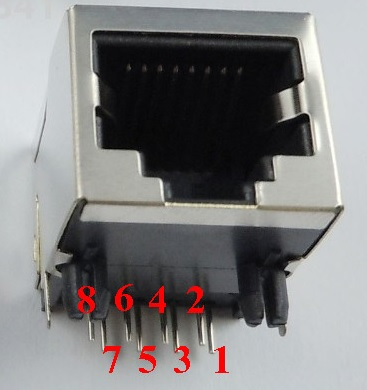
\includegraphics[width=30mm]{Rysunki/Rozdzial3/rj45 jack.jpg}
    \caption{8P8C port line enumeration - Electronics Stack Exchange}
    \label{fig:my_label}
\end{figure}

\begin{figure}[!ht]
    \centering
    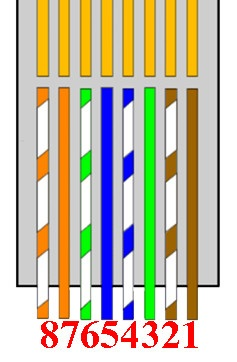
\includegraphics[width=25mm]{Rysunki/Rozdzial3/rj45 plug.jpg}
    \caption{8P8C connector line enumeration - Electronics Stack Exchange}
    \label{fig:my_label}
\end{figure}

The connection between the MAC and the PHY layers is carried out via platform-independent MII interface (\emph{Media-Independent Interface}) or its reduced version RMII (\emph{Reduced Media-Independent Interface}). It takes form of a connection between the processing unit and the Ethernet port driver, equipped with DAC (\emph{Digital-Analog Converter}) and ADC (\emph{Analog-Digital Converter}) in order to allow for transmission via differential signal through the Ethernet cable. Figure 3.6 presents a functional diagram of a sample Ethernet driver, and figure 3.7 its placement in a platform blueprint between MAC and PHY layers.

\begin{figure}[!ht]
    \centering
    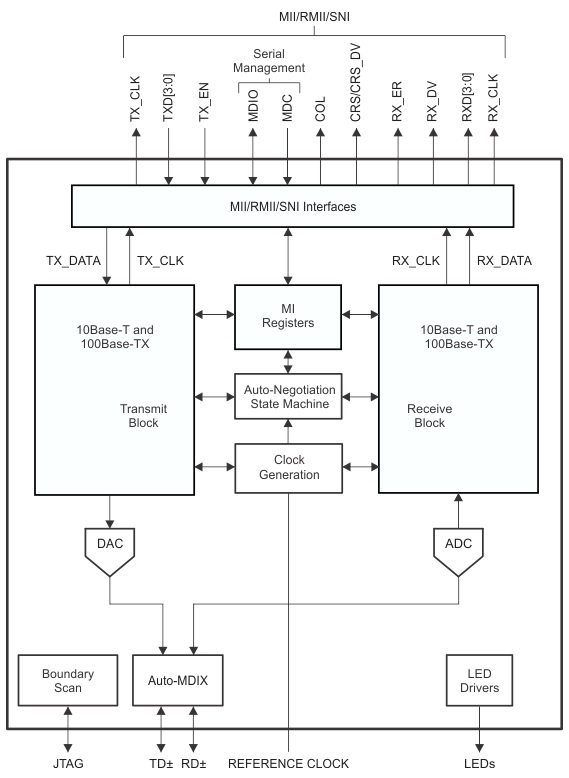
\includegraphics[width=70mm]{Rysunki/Rozdzial3/sterownik-rj45.jpg}
    \caption{Functional diagram of DB83848-P Ethernet driver by Texas Instruments - Texas Instruments}
    \label{fig:my_label}
\end{figure}

\begin{figure}[!ht]
    \centering
    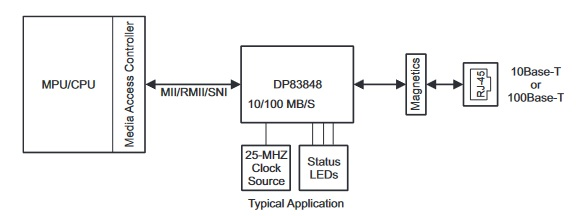
\includegraphics[width=80mm]{Rysunki/Rozdzial3/driverplacement.jpg}
    \caption{DB83848-P driver placement - Texas Instruments}
    \label{fig:my_label}
\end{figure}

The use of RMII allows for connecting different physical mediums (such as UTP cable, fibre optics) to the same data link layer. Table 3.1 describes the lines present in the RMII and their purposes \cite{wiki:rmii}\cite{artykul:rmii}. The MAC abbreviation stands for data link layer, and the PHY abbreviation stands for physical layer.

\begin{table}[!ht]
    \centering
    \caption{RMII lines}
    \begin{tabular}{c|c|c}
        Line designation & Transmission direction & Description  \\
        \hline
        REF\texttt{\char`_}CLK & Any one-way & Reference clock 50 MHz \\
        TXD0 & MAC -> PHY & First transmission bit \\
        TXD1 & MAC -> PHY & Second transmission bit \\
        TX\texttt{\char`_}EN & MAC -> PHY & Transmission start signal \\
        RXD0 & PHY -> MAC & First reception bit \\
        RXD1 & PHY -> MAC & Second reception bit \\
        CRS\texttt{\char`_}DV & PHY -> MAC & Carrier detection line \\
        RX\texttt{\char`_}ER & PHY -> MAC & Reception error line \\
        MDIO & two-way & Administrative data line \\
        MDC & MAC -> PHY & Clock signal for line MDIO
    \end{tabular}
    \label{tab:my_label}
\end{table}

Transmitting via RMII requires converting the binary representation of the code of sent character to big-endian notation, which even index bits (starting enumerating from 0) are transmitted via line TXD0, and odd index bits via line TXD1, creating so called \emph{di-bit} or \emph{nibble} transmission. Similarly to the transmission, reception of the data happens by receiving bits with even index (with enumerating from 0) on line RXD0 and bits with odd indexes on line RXD1.

The connection of lines within the UTP cables for the 8P8C connectors is an important matter. In case of connecting two devices deemed as \emph{hosts}, it is necessary to use a crossover cable, which is a cable where the transmitting and receiving pair between each end of the cable are switched. However in case of connecting a host to a device such as a router (which has an on-board switch), a straight-thru cable needs to be used. Those two ways of making the 8P8C connector for the UTP cable are known as T-568A and T-568B respectively.

\begin{figure}[!ht]
    \centering
    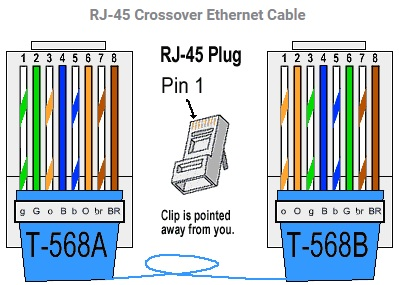
\includegraphics[width=54mm]{Rysunki/Rozdzial3/cross.jpg}
    \caption{Line placement in UTP cable - The Internet Centre Inc.}
    \label{fig:my_label}
\end{figure}

\newpage
\subsection{Wireless connectivity}

Thanks to the popularity of integration of embedded systems with wireless networks, especially in case of home and office automation, the market offers a number of different modules providing wireless network functionalities, both for Wi-Fi and cellular data. Due to their very similar construction, in which the major difference often is only the type of antenna for given frequency, this thesis provides only a general description of said modules.

Majority of the modules are available in the form of preprogrammed digital circuits on a PCB board, most commonly with integrated mocroband antenna (in form of a path on the printed board), with SMA antenna port used for concentric cables, IPEX port, or u.FL port. Figure 3.7 presents example antennas used by wireless modules.

\begin{figure}[!ht]
    \centering
    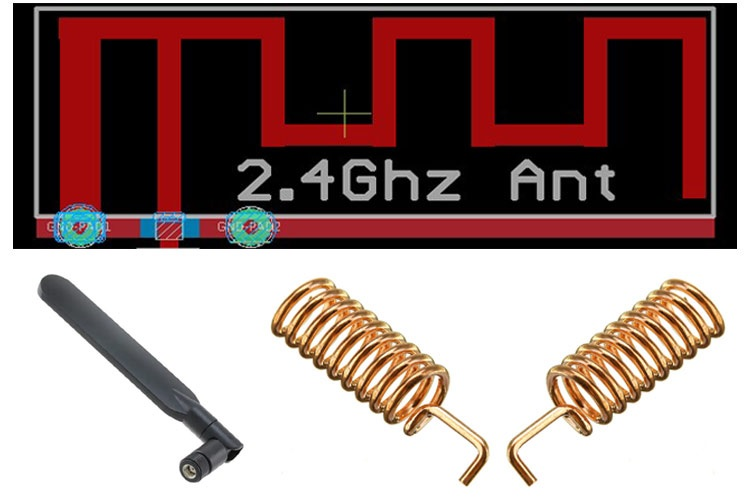
\includegraphics[width=45mm]{Rysunki/Rozdzial3/antenna.jpg}
    \caption{Antenna types for embedded systems - Circuit Digest}
    \label{fig:my_label}
\end{figure}

Part of the circuits which implement the wireless interface are available in a form of a Shield extension, which allows for very easy integration with Arduino hardware platform, without the need for soldering. The construction of such module is very similar to the Arduino hardware platform itself, having ports that are corresponding with function and placement to the ones present on the microcontroller board. In case of modules which offer the GSM connectivity, it is necessary to additionally provide a SIM card, similarly to the common mobile phones.

\begin{figure}[!ht]
\begin{minipage}[b]{0.4\textwidth}
    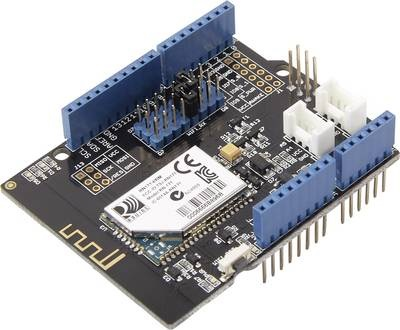
\includegraphics[width=60mm]{Rysunki/Rozdzial3/shield.jpg}
    \caption{Wi-Fi Shield - Seeed Studio}
  \end{minipage}
  \hfill
  \begin{minipage}[b]{0.4\textwidth}
    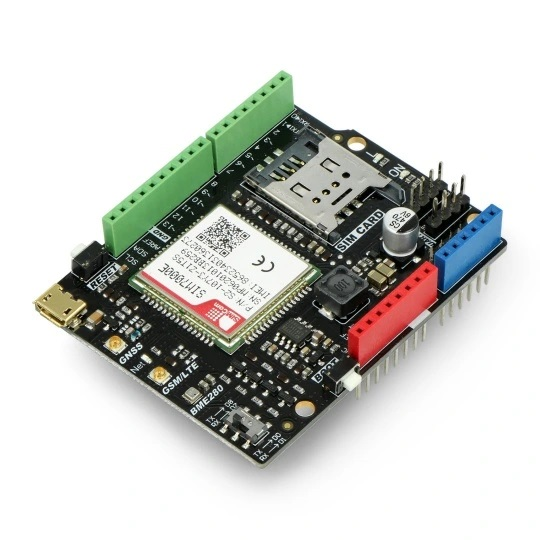
\includegraphics[width=60mm]{Rysunki/Rozdzial3/gsm.jpg}
    \caption{GSM Shield - Botland}
  \end{minipage}
\end{figure}

\newpage
\section{TCP/IP stack implementation}

Implementation of TCP/IP stack, both due to the number and the complexity of the protocols, is a complex task. Because of that, the most common approach is to use already established solutions. Some of the devices (especially extension modules) implement the whole TCP/IP stack, requiring from the user only implementing the communication with selected local serial interface, such as SPI or I$^2$C.

\begin{figure}[!ht]
    \centering
    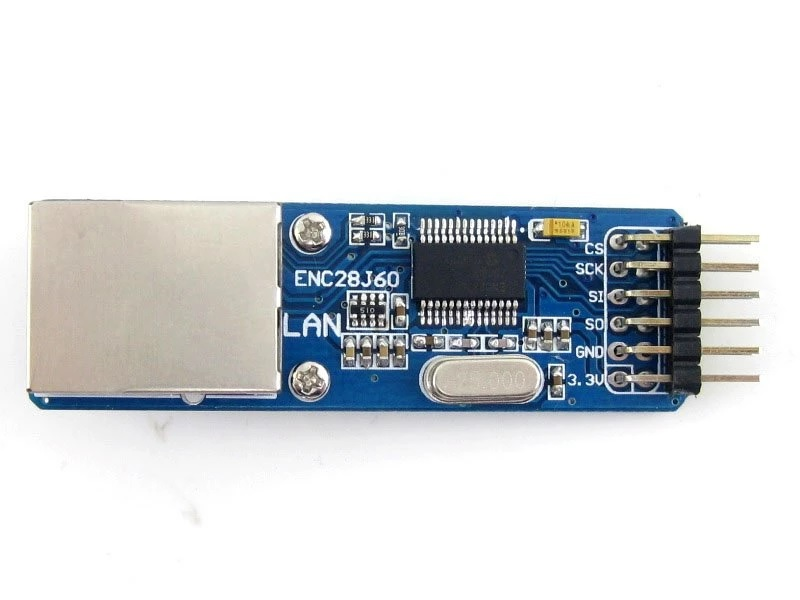
\includegraphics[width=60mm]{Rysunki/Rozdzial3/enc28j60.jpg}
    \caption{ENC28J60 module - Aliexpress}
    \label{fig:my_label}
\end{figure}

ENC28J60 module \cite{enc28j60} is an example of solution providing an external Ethernet interface, which was shown on figure 3.12. It has compatibility with 10/100/1000Base-T networks, supporting especially 10Base-T transmission. In order to communicate with a microcontroller, and SPI interface with the clock frequency of 20 MHz is used. It provides only the implementation of physical and data link layer of the OSI model, which forces the user to implement the other layers of the TCP/IP stack on their own. Said module possesses an 8kB programmable memory for reception and transmission buffers and hardware control sum calculation. Thanks to implementing the application layer on the microcontroller, the amount of available network logical sockets is entirely dependent on the RAM memory size of the microcontroller.

\begin{figure}[!ht]
    \centering
    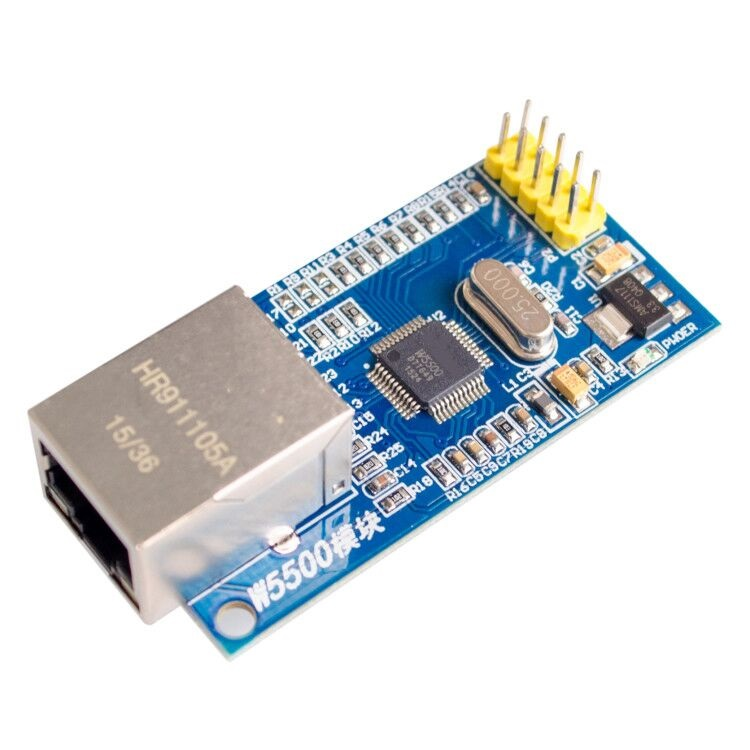
\includegraphics[width=60mm]{Rysunki/Rozdzial3/w5500.jpg}
    \caption{W5500 module - Aliexpress}
    \label{fig:my_label}
\end{figure}

W5500 is another example of wired connectivity as shown on figure 3.13. On contrary to the ENC28J60 module, it offers also part of the higher layers protocols, such as TCP, UDP, ICMP, IPv4, ARP, IGMP and PPPoE \cite{w5500}. Additionally it provides the functionality of \emph{wake on LAN}. This module is also available in the form of Shield extension for the Arduino boards. It operates with standards 10/100 Base-T and contains 32 kB programmable memory for transmission and reception buffers, and supports 8 logical network sockets. The module operates with 3.3 V power level, while tolerating 5 V on the I/O (Input/Output) pins. Table 3.2 presents the comparison of aforementioned modules with reference prices. 

\begin{table}[!ht]
    \centering
    \caption{Ethernet module parameters comparison}
    \begin{tabular}{c|c|c|c|c|c}
        \multirow{2}{*}{Module} & Standard & \multirow{2}{*}{Protocols} & \multirow{2}{*}{Interface} & Speed & \multirow{2}{*}{Price} \\
        & Transmission & & & Interface \\
        \hline
        ENC28J60 & 10Base-T & MAC & SPI & 20 MHz & 32.70 PLN \\
        \hline
        \multirow{3}{*}{W5500} & \multirow{3}{*}{10/100Base-T} & MAC, TCP, UDP, & \multirow{3}{*}{SPI} & \multirow{3}{*}{80 MHz} & \multirow{3}{*}{115.00 PLN} \\
        & & ICMP, IPv4, ARP, & & & \\
        & & & IGMP, PPPoE & &
    \end{tabular}
    \label{tab:my_label}
\end{table}

Two of the most popular wireless connectivity modules are ESP8266 and ESP32, presented by figures 3.14 and 3.15 respectively. The later module is a newer version of the former one. Both of the modules operate in 2.4 GHz band, with the IEEE 802.11 b/g/n standards. They differ in available speeds, security features and serial interfaces providing connection with the microcontroller. Both modules use pad and THT connectors, allowing the user to solder in the goldpin pins. Both ESP8266 and ESP32 can operate in the softAP (\emph{Soft Access Point}) mode and as a transceiving station (\emph{STA}).

\begin{figure}[!ht]
\begin{minipage}[b]{0.4\textwidth}
    \centering
    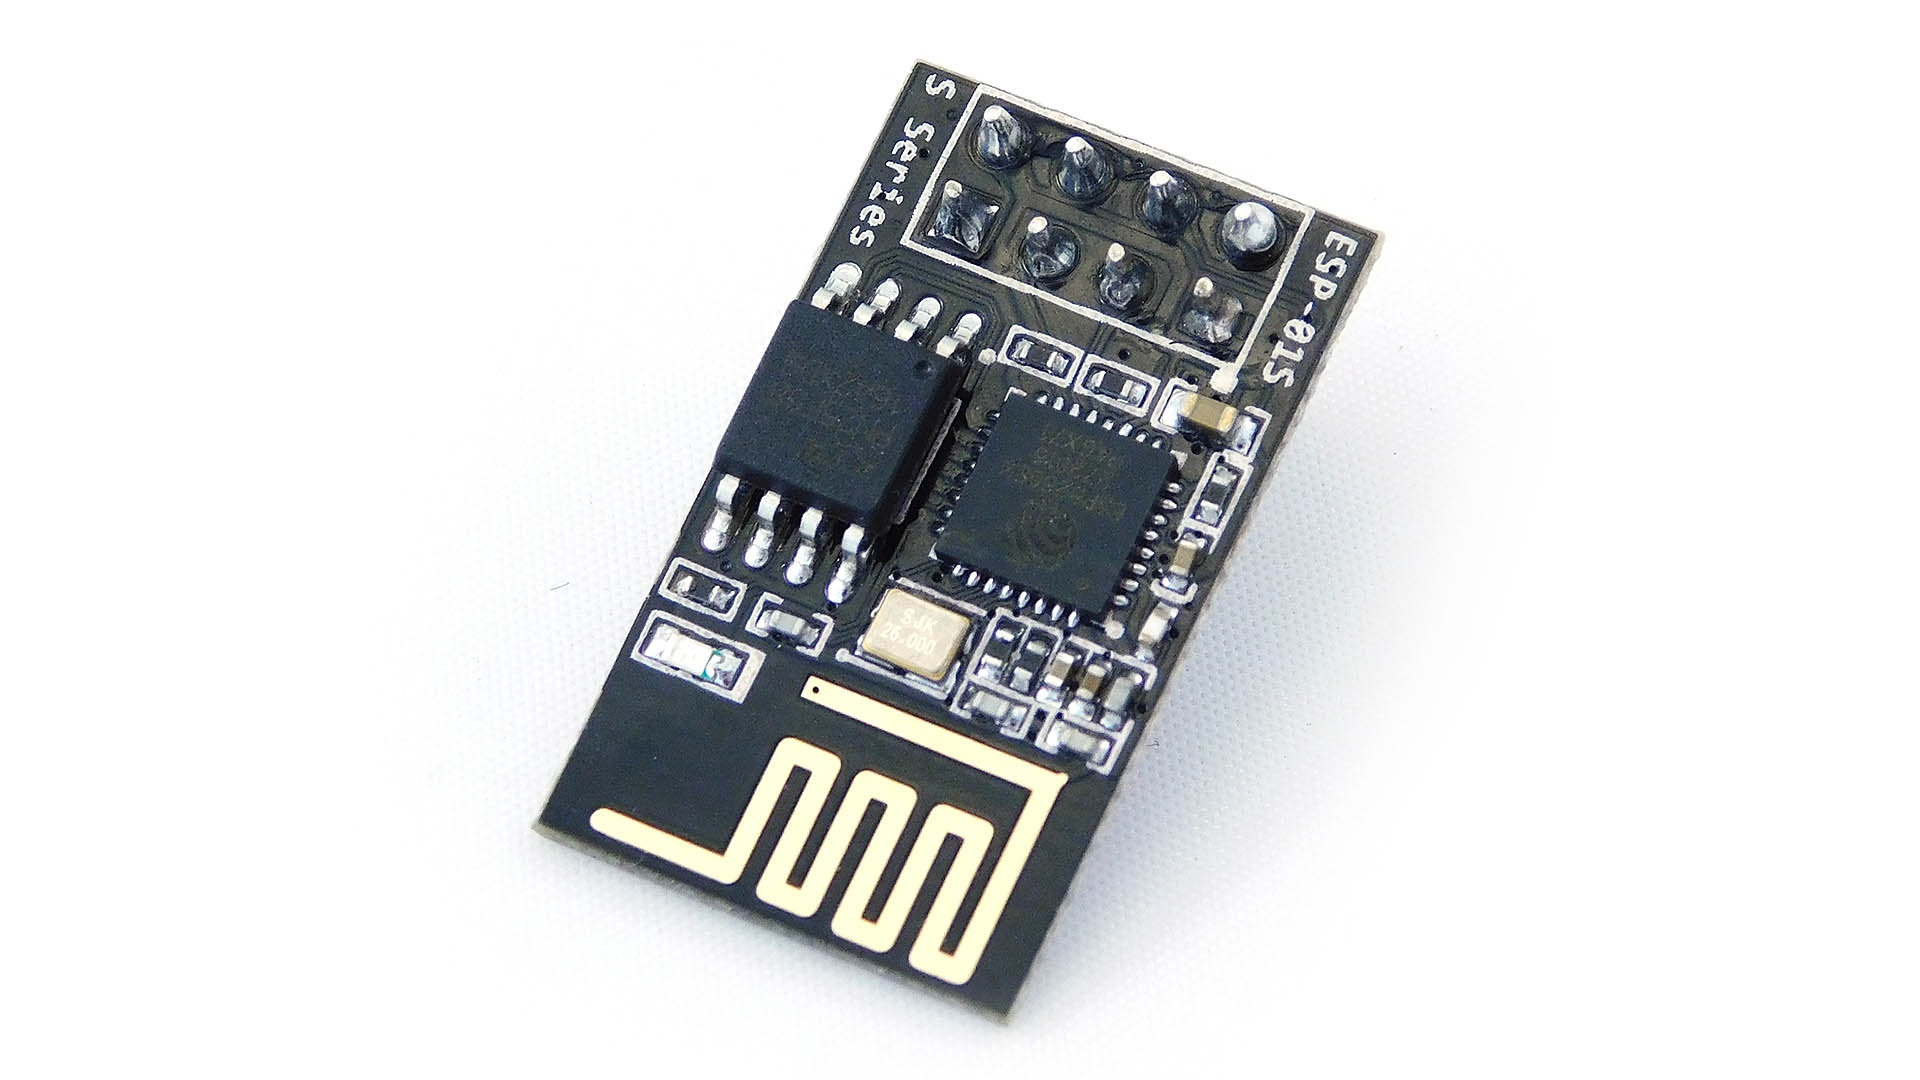
\includegraphics[width=70mm]{Rysunki/Rozdzial3/esp8266.jpg}
    \caption{ESP8266 module - Nettigo}
  \end{minipage}
  \hfill
  \begin{minipage}[b]{0.4\textwidth}
    \centering
    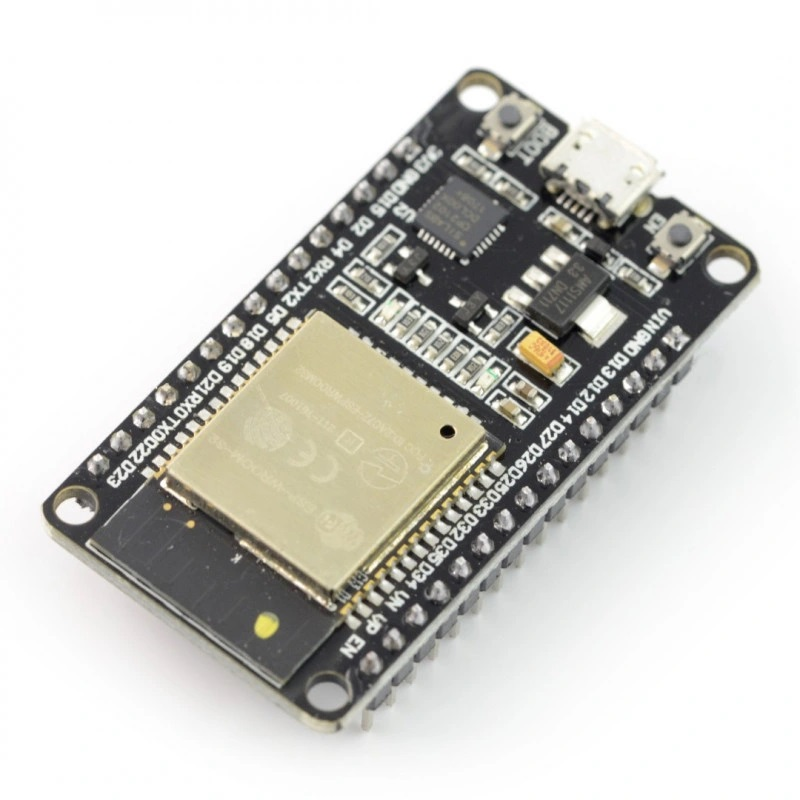
\includegraphics[width=40mm]{Rysunki/Rozdzial3/esp32.jpg}
    \caption{ESP32 module - Botland}
  \end{minipage}
\end{figure}

ESP8266 provides the communication speed up to 72.2 Mbps. \emph{Firmware} delivered by the module manufacturer implements IPv4, TCP, UDP, HTTP, ICMP and MAC protocols and offers encryption via WEP, WPA/WPA2, TKIP and AES algorithms \cite{esp8266}. In order to communicate with microcontroller, it uses the UART (\emph{Universal Asynchronous Receiver Transmitter}) interface, and uses AT commands in order to control the module. Its operating voltage is around 3.3 V, and two antenna types are available - a microband integrated antenna, or an u.FL port.

ESP32 is a newer version or said ESP8266. The circuit contains a dual core processing unit, which allowed for increasing the transmission speed up to 150 Mbps \cite{esp32}. Similarly to ESP8266, the manufacturer provides \emph{firmware} which implements IPv4, TCP, UDP, HTTP, ICMP and MAC protocols, but has more extensive security features, extending the encryption algorithm range by PSK/Enterprise, SHA-2, ECC and RSA-4096 algorithms. Some of the variants of the module have integrated support for IPv6 protocol. There is a possibility for the user to create their custom version of said firmware, containing protocols suited for their needs, using the SDK (\emph{Software Development Kit}) provided by the manufacturer. The module operates with the voltage of 3.3 V. In order to communicate with the microcontroller, user can use either SPI, I$^2$C or UART interfaces. Table 3.3 shows the comparison of the parameters of the modules along with their reference prices.

\begin{table}[!ht]
    \centering
    \caption{Overview of wireless modules parameters}
    \begin{tabular}{c|c|c|c|c|c}
        \multirow{2}{*}{Module} & Standard & \multirow{2}{*}{Protocol} & \multirow{2}{*}{Interface} & Speed & \multirow{2}{*}{Price} \\
        & of transmission & & & of transmission \\
        \hline
        \multirow{2}{*}{ESP8266} & \multirow{2}{*}{802.11 b/g/n} & MAC, TCP, UDP, & \multirow{2}{*}{UART} & \multirow{2}{*}{72,2 Mbps} & \multirow{2}{*}{14.90 PLN} \\
                & & HTTP, IPv4, ICMP & & & \\
        \hline
        \multirow{3}{*}{ESP32} & \multirow{3}{*}{802.11 b/g/n} & MAC, TCP, UDP, & \multirow{2}{*}{SPI, I$^2$C,} & \multirow{3}{*}{150 Mbps} & \multirow{3}{*}{127.50 PLN} \\
        & & HTTP, IPv4, (IPv6), & \multirow{2}{*}{UART} & & \\
        & & ICMP & & &
    \end{tabular}
    \label{tab:my_label}
\end{table}

\begin{figure}[!ht]
    \centering
    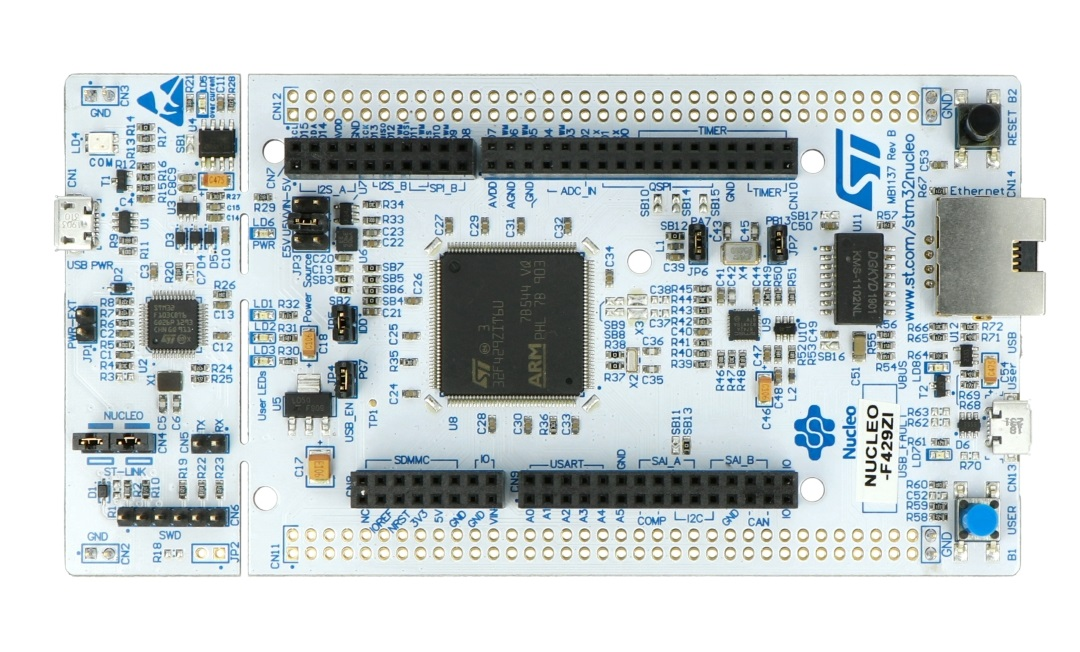
\includegraphics[width=100mm]{Rysunki/Rozdzial3/nucleo.jpg}
    \caption{Nucleo-F429ZI platform with integrated Ethernet port \dywiz{} Botland}
    \label{fig:my_label}
\end{figure}

Some of the manufacturers of hardware platform decide to partially implement the TCP/IP stack for their platforms in cases, when they are equipped with integrated network interface (such as 8P8C port). Nucleo-F4 are a good example of such platforms (eg. Nucleo-F429ZI board shown by figure 3.16) equipped with integrated 8P8C port. The HAL (\emph{Hardware Abstract Layer}) software distributed by the ST Microelectronics for said microcontrollers provides the implementation of the network access layer, however it does not offer the higher layers, requiring the user to utilize middleware, such as eg. open source LwIP (\emph{Lightweight IP}) or uIP (\emph{micro IP}) stacks. In order to use the said protocol stacks, they need to be ported first for given microcontroller, or the user needs to use an already available solution if it has been created so far.

The LwIP stack contains the implementation of protocols of application, transport and network layer. Those protocols are as follows \cite{lwip:protocols}:

\begin{itemize}
    \item [1)] IP;
    \item [2)] ICMP;
    \item [3)] UDP;
    \item [4)] DHCP;
    \item [5)] TCP;
    \item [6)] ARP;
    \item [7)] BSD (optionally)
\end{itemize}

Since version v.2.0.0 the LwIP stack supports both IPv4 and IPv6 addressing. 

uIP is an open-source implementation of the TCP/IP stack dedicated for microcontrollers with very limited Flash and RAM memory. According to the document \cite{ti:uip} the uIP stack can minimize the RAM usage to a couple hundred bytes. It implements the following protocols:

\begin{itemize}
    \item [1)] TCP;
    \item [2)] UDP;
    \item [3)] IP;
    \item [4)] ICMP;
    \item [5)] ARP
\end{itemize}

Due to very harsh requirements regarding memory optimization, all application layer protocols are left for implementation by the user. This decision was also made in part due to being unable to predict what specific applications the stack will be used for.